\section{Mode shape: a cross-section field, and a comparison that was wrong}
\label{sec:modes}

% TODO: full chapter --- reader: an engineer who wants to know whether the extracted
% cross-section field is the mode the analytic basis describes; test: they can compare
% Figure~\ref{fig:mode-shape-mispaired} with Figure~\ref{fig:mode-shape-corrected} panel
% for panel, see that only the e_z row changes, and check the printed correlations against
% the audit table. PLACEHOLDER: captions and figures only, no chapter prose. Still to
% write: why the longitudinal and the vertical component are different objects, what
% e_z_superseded measures physically, and what the residual rim at the strip edges and
% the substrate interface says about the discretisation.

\begin{figure}[H]
  \centering
  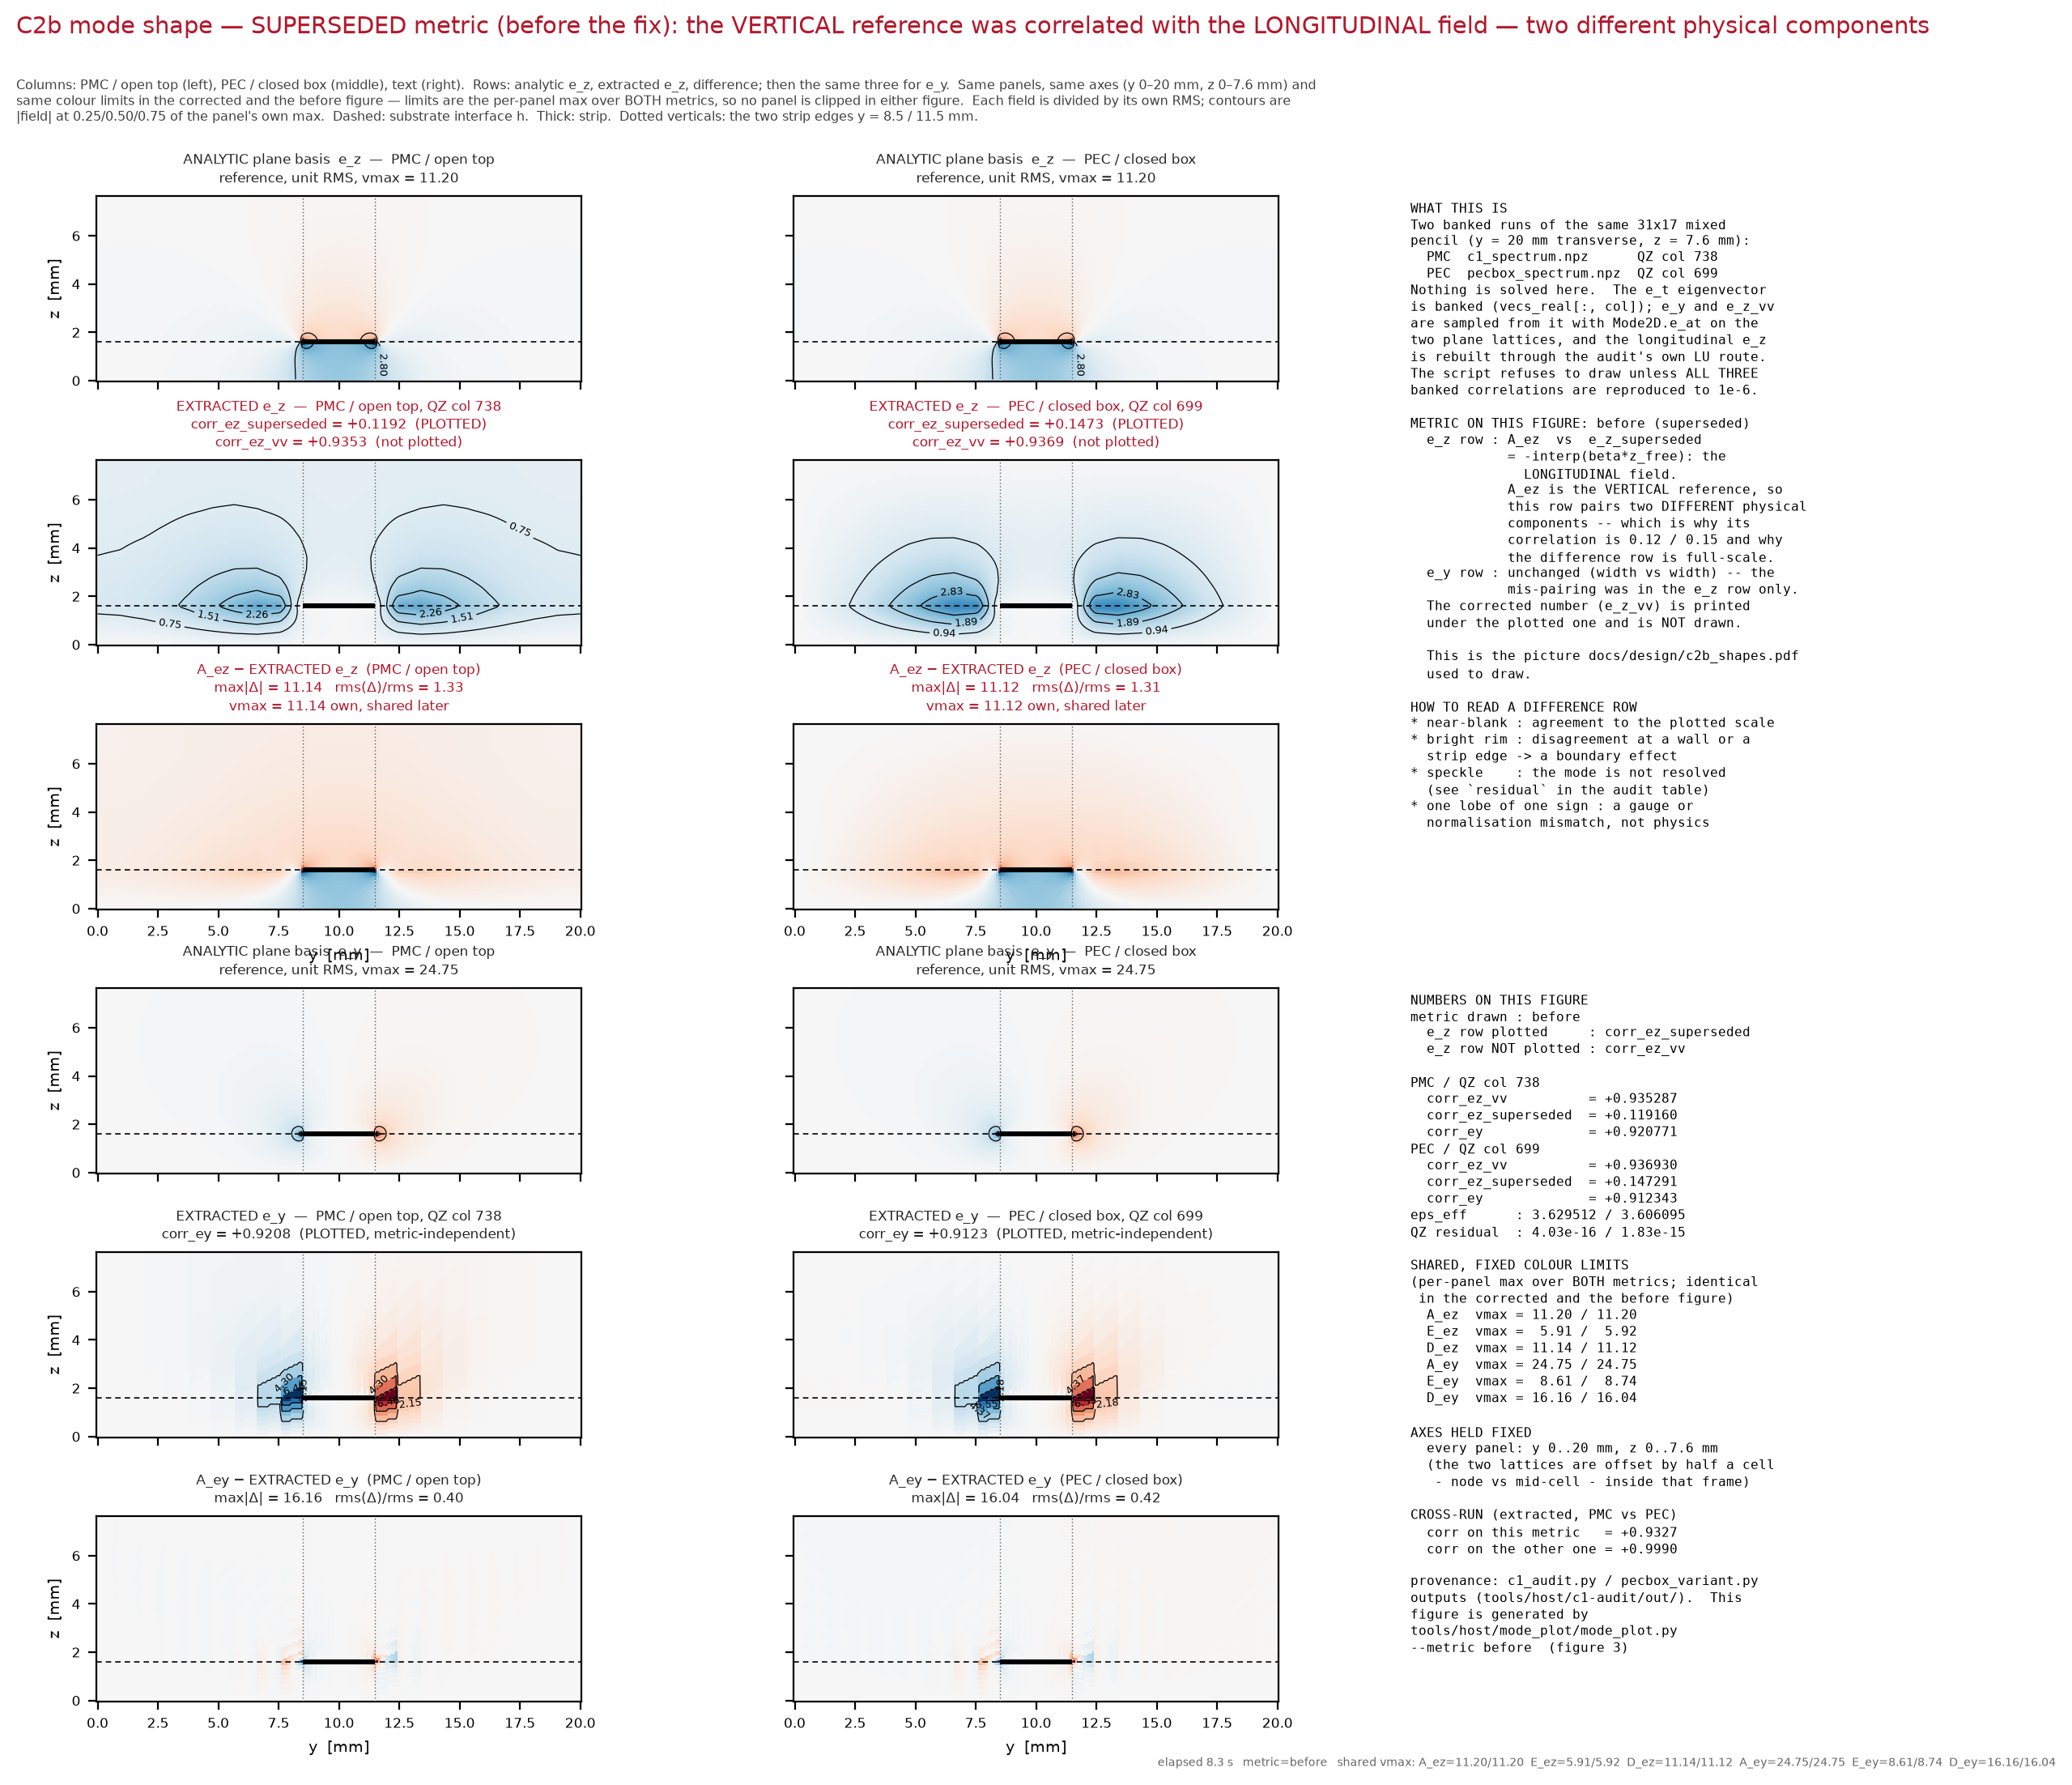
\includegraphics[width=0.95\textwidth]{../figures/mode_shape_mispaired_before.png}
  \caption[The superseded comparison: an analytic vertical reference correlated with an extracted longitudinal field.]{The
  superseded comparison. The $e_z$ row correlates two arrays that were never the same quantity: the analytic
  \emph{vertical} reference against the extracted \emph{longitudinal} field,
  $e_{z,\text{superseded}} = -\mathrm{interp}(\beta z_{\text{free}})$, on both banked runs (PMC QZ column $738$ of
  \texttt{c1\_spectrum.npz}, PEC QZ column $699$ of \texttt{pecbox\_spectrum.npz}, both $31\times17$). It reads
  $\mathrm{corr} = +0.1192$ (PMC) and $+0.1473$ (PEC), and the difference rows are correspondingly full-scale,
  $\max|\Delta| = 11.14$ and $11.12$ with $\mathrm{rms}(\Delta)/\mathrm{rms} = 1.33$ and $1.31$: the residual is
  larger than the field. The arithmetic is not wrong here, the \emph{pairing} is — a small correlation is the
  correct answer to a meaningless question, and that is why this row must not be read as the mode failing. \par
  The $e_y$ row is the built-in control: width against width, untouched by the mis-pairing, $\mathrm{corr} =
  +0.9208$ (PMC) and $+0.9123$ (PEC), drawn identically to the same row of
  Figure~\ref{fig:mode-shape-corrected}. The correct statistic for the $e_z$ row is printed beneath the plotted
  number on each extracted panel and is deliberately not drawn: $+0.9353$ and $+0.9369$.}
  \label{fig:mode-shape-mispaired}
\end{figure}

\begin{figure}[H]
  \centering
  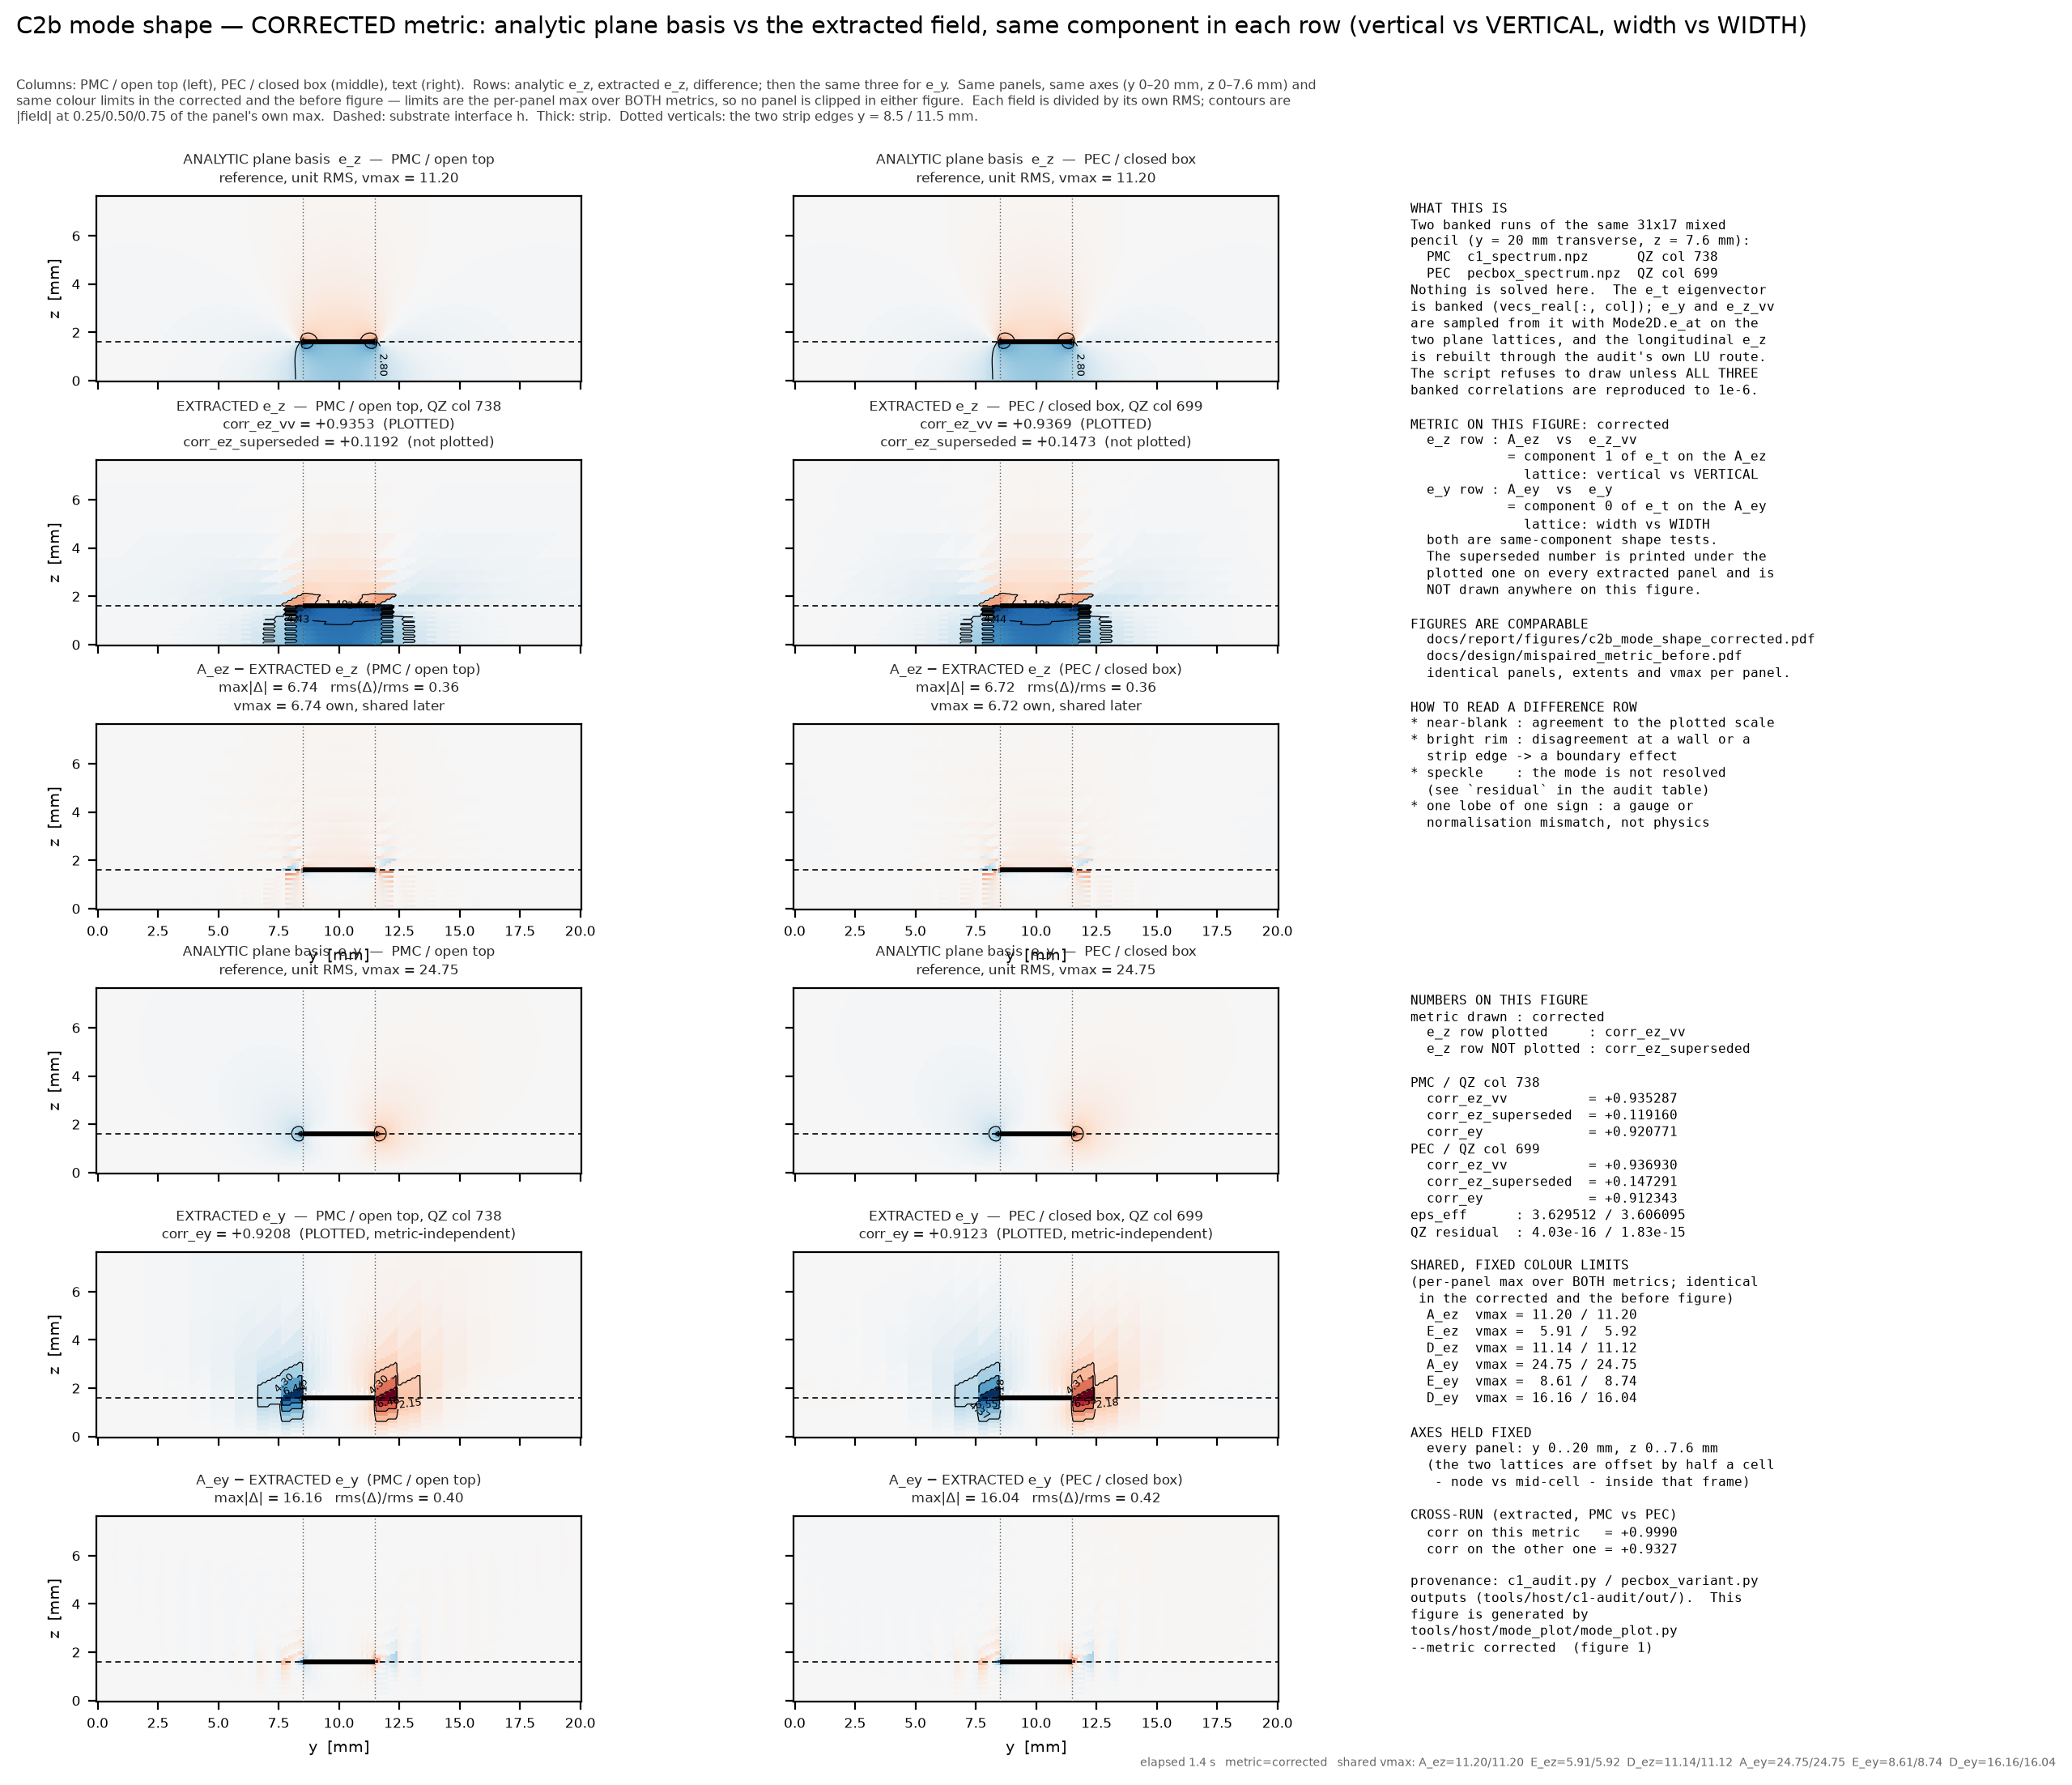
\includegraphics[width=0.95\textwidth]{../figures/mode_shape_corrected.png}
  \caption[The corrected comparison: the same components paired vertical with vertical.]{The corrected
  comparison: same banked runs, same panels, same extents, same per-panel colour limits, one row redrawn. The
  $e_z$ row now pairs like with like — component~$1$ of the banked $e_t$ eigenvector sampled on the
  $A_{ez}$ lattice against the analytic vertical reference, vertical versus vertical — and it reads
  $\mathrm{corr} = +0.9353$ (PMC) and $+0.9369$ (PEC). The difference rows fall to $\max|\Delta| = 6.74$ and
  $6.72$ with $\mathrm{rms}(\Delta)/\mathrm{rms} = 0.36$, and the two runs agree with each other on this metric at
  $+0.9990$ against $+0.9327$ on the superseded one. The reader's rule that this pair exists to teach: read which
  two things are being paired before believing which number. \par
  What the difference rows show is a near-blank field with a bright rim at the strip edges and at the substrate
  interface — disagreement concentrated where the discretisation is thinnest and where the reference field has its
  largest gradient, a boundary effect rather than a shape error. Because every extent and every per-panel limit is
  shared with Figure~\ref{fig:mode-shape-mispaired}, the two pages can be flipped between directly and any
  difference seen between them is the metric and nothing else.}
  \label{fig:mode-shape-corrected}
\end{figure}
